\subsection{Machine learning Methods}
This section describes the classification methods used in this study. Each represents a different approach within supervised learning.

\subsubsection{Pre processing and Data Augmentation}
\label{sec:preprocessing}
To implement the methods based on Machine learning or deep learning for hate speech detection on Twitter, a thorough data preprocessing procedure was carried out to balance the classes in the dataset. First, the two target categories were identified: \textit{hate speech} and \textit{no hate speech}, encoded as 1 and 0, respectively. Various text cleaning techniques were then applied, including the removal of special characters, URLs, mentions, Twitter-specific symbols, spelling correction, stopword removal, stemming, as well as the elimination of duplicate records and null values. Additionally, the vocabulary was enriched through synonym validation and expansion. To address the inherent class imbalance, the Easy Data Augmentation (EDA) technique was applied, which allowed for the generation of a balanced dataset, ultimately saved in a CSV file named \texttt{balanced\_data.csv}~\cite{wei2019eda}.

The preprocessing approach adopted in this study shares several similarities with previous works such as those by Fieri et al.~\cite{fieri2023offensive} and Almeida et al.~\cite{almeida2023comparison}, particularly in terms of text data cleaning and preparation for hate speech detection tasks. As in these studies, common techniques were applied, including the removal of textual noise (mentions, URLs, symbols), lexical normalization, and dimensionality reduction through the use of stopwords and stemming. However, our approach integrates additional steps that are not consistently addressed in those works, such as automated spelling correction, semantic validation using synonyms, and the application of data augmentation techniques like Easy Data Augmentation (EDA). This last aspect represents a significant difference, as the reviewed studies often rely on direct undersampling or oversampling, whereas our methodology emphasizes the synthetic generation of new samples. This can contribute to greater dataset diversity and model robustness during training, regardless of the architecture employed~\cite{wei2019eda}.


\subsection{Logistic Regression}
\subsubsection{Definition}
Logistic regression is a statistical model used to predict the probability of a binary class. It is efficient for linear problems and serves as a baseline for comparison with more complex models.

To reference one of the earliest formulations of the model, we draw upon the perspective presented in \textit{The Regression Analysis of Binary Sequences} by D. R. Cox (1958), which introduced a rigorous statistical framework for the analysis of binary outcomes. In this work, both dependent and independent variables are explicitly identified, and the probability of a binary event is modeled using a logistic transformation of the predictors. Dependent variables are represented as binary categorical variables, typically coded as 0 and 1, which enables the analysis of how one or more explanatory variables influence the likelihood of an event of interest. Through illustrative examples, the author demonstrates how the model can be estimated using maximum likelihood methods, thereby establishing a methodological foundation that continues to be widely applied in fields such as biostatistics, the social sciences, and machine learning \citep{cox1958logistic}.

Given the capabilities offered by the model, it has been selected for use in this study. However, prior to its implementation, we will review some previous approaches used in earlier research.

As one of the initial and relevant approaches, the study presented in the article "Offensive Language Detection Using Soft Voting Ensemble Model" \citep{supert2023offensive} incorporates logistic regression as part of its ensemble strategy. The article emphasizes the use of L2 regularization, which enhances the precision of offensive language classification by mitigating overfitting. Furthermore, the model's simplicity is highlighted as a significant advantage, enabling efficient implementation even with limited computational resources—demonstrating its usefulness and versatility within the set of evaluated classifiers.

The research article titled "Comparison between Machine Learning and Deep Learning Approaches for the Detection of Toxic Comments on Social Networks" \citep{bonetti2023comparison} employs logistic regression once again, combining it with two semantic modeling techniques: Latent Semantic Analysis (LSA) and Latent Dirichlet Allocation (LDA). These methods will be further discussed in the following paragraphs. Notably, the study reports a prediction accuracy exceeding 91%, highlighting the competitiveness of traditional approaches compared to more complex deep learning models.



\subsection{Deep Learning Methods}
Deep learning is a subset of machine learning that uses artificial neural networks with many layers to automatically learn complex patterns from large amounts of data.

\subsubsection{roBERTa}
RoBERTa is a bidirectional pretrained encoder based on BERT, but trained on a larger amount of data and with longer sequences. BERT itself is based on the encoder component of the Transformer architecture, which generates vector representations by considering both the past and future context of the sequence elements. The pretrained knowledge of the model can be reused for other tasks by simply adding a classification head and fine-tuning the pretrained weights to solve the new problem. In \cite{bonetti2021hate}, BERTweet was used — a model similar to RoBERTa but specifically trained on Twitter data — achieving an accuracy of 92.38.

\subsubsection{Methodology XGBoost}

The methodology used for the XGBoostClassifier began by loading the [CLS] token embeddings generated by RoBERTa, that is, the vector that summarizes the entire text sequence. After this, the data was split into 80\% for training and 20\% for testing. This split resulted in 38,152 examples available for training. Subsequently, a parameter grid was defined to conduct hyperparameter tuning. The search focused on the number of estimators, maximum tree depth, and minimum child weight. To find the best values, a grid search with 3-fold cross-validation was used.

In addition to this search, other hyperparameters were set manually. For example, 80\% of the data was used in each boosting round, and in each tree and node, a sample of features was selected such that its size was proportional to the square root of the total number of features, as recommended in \cite{Chen2016XGBoost}.

For training, 50\% of the dataset was used to perform the hyperparameter search, as doing it on the entire training set would have been computationally too expensive. Once the best hyperparameters were found, the model was trained on the full training set and then evaluated.

To evaluate the model, a classification report was generated that measured precision, recall, F1-score, and accuracy. Additionally, a confusion matrix was presented to more clearly observe the trend of the data toward true positives or misclassification.

\subsubsection{Methodology BI-LSTM}

For the model based on the BI-LSTM architecture, the full embeddings generated by the roBERTa model were used, and the architecture shown in Figure~\ref{fig:bilstm_architecture}, as recommended in \cite{zhang2018deep}, was implemented. This architecture was trained using the Adam optimizer for 200 epochs, storing the checkpoint that achieved the highest accuracy on the validation set. This validation set accounted for 15\% of the data, as did the test set, while the remaining 70\% was used for training. 

After training, the best checkpoint was restored and performance evaluation was carried out. The model was assessed using the same metrics as with the XGBoostClassifier: precision, recall, F1-score, accuracy, and the confusion matrix.

\begin{figure}[htbp]
  \centering
  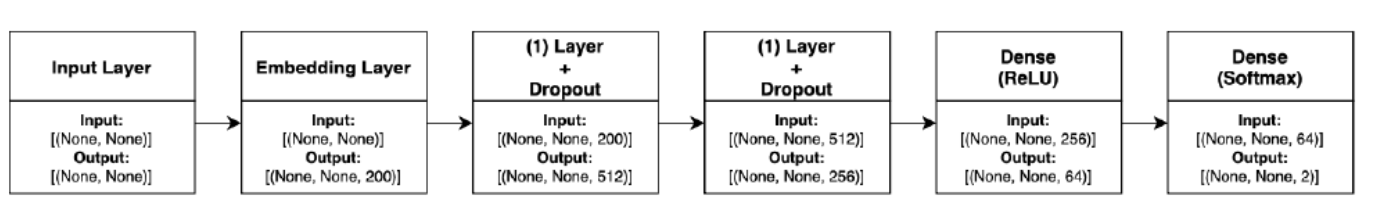
\includegraphics[width=0.45\textwidth]{images/bilstm_architecture.png}
  \caption{BI-LSTM architecture used in the model.}
  \label{fig:bilstm_architecture}
\end{figure}

\subsubsection*{Fine-tuning methodology for RoBERTa}

To fine-tune the pretrained \texttt{twitter-roBERTa} model and adapt it to solve the classification task, we used the tokenized input data, which had not yet been embedded by the model. These data were split into 70\%, 15\%, and 15\% for the training, validation, and test sets, respectively, similar to the BI-LSTM architecture. 

Next, we created a three-layer classification head following the architecture shown in Figure~\ref{fig:roberta_finetune_architecture} \cite{liu2019roberta}. Dropout layers were added to prevent overfitting. This classification head was then integrated with the RoBERTa encoder, using the representation of the \texttt{[CLS]} token, which, as mentioned before, summarizes the input sequence.

With the full model ready, we froze the RoBERTa weights to train only the classification head. The training lasted 150 epochs, used batches of 32 samples, and employed the Adam optimizer, storing the checkpoints of the best-performing models. After this first stage, we evaluated the results and performed a second training stage, where all pretrained weights were unfrozen. This second stage was trained using a learning rate of 0.000001, the Adam optimizer, for 100 epochs, again with a batch size of 32.

To assess the best model from each training stage as well as the untrained model, we used precision, recall, F1-score, accuracy, and the confusion matrix.

\begin{figure}[htbp]
  \centering
  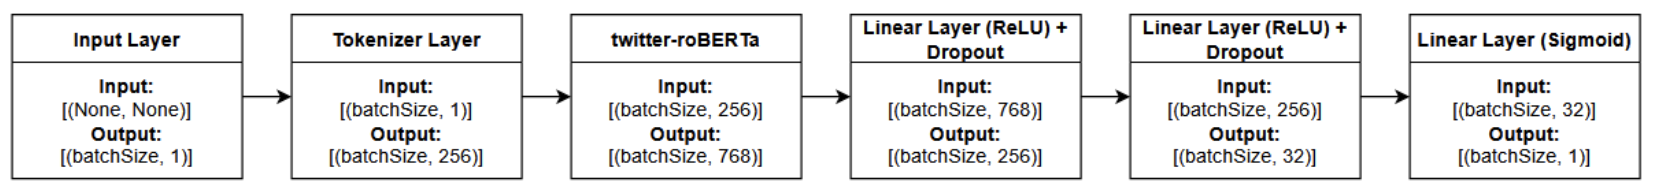
\includegraphics[width=0.45\textwidth]{images/roberta_finetune_architecture.png}
  \caption{Architecture used for fine-tuning twitter-RoBERTa.}
  \label{fig:roberta_finetune_architecture}
\end{figure}


\subsubsection{BI-LSTM}

\noindent
\cite{toktarova2023hate} BI-LSTM (Bidirectional Long Short-Term Memory) is a type of sequential neural network that allows working with data composed of different elements ordered in a sequence, such as text. This type of network can make predictions about parts of the sequence based on what has been seen so far or on the entire input. It is an improvement over LSTM networks, which, like recurrent networks, use output values from previous steps in the sequence. However, it differs by dividing the network's responsibilities into different flow control gates. Additionally, it is capable of maintaining both long-term memory and a hidden state, which allows it to respond appropriately to the current step in the sequence. BI-LSTMs process the input both forward and backward, thus capturing future and past context at each step. In \cite{fieri2021soft}, using BI-LSTM, an accuracy of 90.2 was achieved; meanwhile, in \cite{bonetti2023comparison}, 96.102 was reached.




\subsubsection{CNN Methodology}
\label{sec:cnn}

Using the Convolutional Neural Network (CNN) architecture, various configurations were explored to obtain an effective training setup. With a balanced dataset of 47,706 labeled messages now available, the data was split into two subsets: 80\% for training and 20\% for testing. The final model was structured with three hidden convolutional layers. Although deeper architectures were initially tested, they were deemed suboptimal given the relatively limited size of the dataset.

Each of the convolutional layers was followed by a ReLU (Rectified Linear Unit) activation function. ReLU is commonly used in deep learning because it introduces non-linearity by outputting zero for all negative values and keeping positive values unchanged, which helps avoid vanishing gradient problems and accelerates convergence.

To reduce the spatial dimensions and computational complexity of the model, a \texttt{MaxPooling1D} layer with a pool size of 2 was applied after each convolution. Max pooling extracts the most prominent feature within each segment of the input, effectively downsampling the representation and providing translation invariance, which is particularly useful in textual pattern recognition.

In order to prevent overfitting—an issue often encountered when training deep networks on relatively small datasets—Dropout layers with a dropout rate of 0.3 were included. Dropout randomly deactivates a fraction of neurons during training, which helps the model generalize better by discouraging co-adaptations of feature detectors.

Finally, the architecture concluded with a dense output layer using the sigmoid activation function. This function maps the output to a probability between 0 and 1, suitable for binary classification tasks like distinguishing between hate and non-hate speech.

The model was compiled and trained using the Adam optimizer, which combines the advantages of both AdaGrad and RMSProp by adapting the learning rate for each parameter. A learning rate of 0.0005 was selected to balance the speed of convergence with training stability, allowing the model to make gradual improvements without overshooting minima.

The implemented CNN model consists of three convolutional blocks followed by max pooling and dropout layers. This structure enables the progressive extraction of textual features while controlling overfitting. The Conv1D layers increase in complexity (from 64 to 256 filters), while MaxPooling1D reduces the dimensionality of the text, making processing more efficient.

The use of Dropout layers between convolutional blocks, with a dropout rate of 0.3, effectively mitigates overfitting—an important consideration given the dataset size of 47,706 samples. Subsequently, a Flatten layer transforms the three-dimensional output into a vector, which is then processed by a dense layer of 128 neurons. This dense layer accounts for the majority of the model’s parameters. Finally, a Dense output layer with a sigmoid activation function performs the binary classification.

Compared to previous studies such as those by Fieri et al. and Almeida et al., this CNN model opts for a lighter architecture focused on efficiency and local pattern extraction, avoiding more complex hybrid or recurrent architectures that are typically more computationally expensive.

During the CNN training phase, an early stopping strategy was implemented to prevent overfitting and optimize generalization. Training was initially scheduled for 30 epochs with a batch size of 32. Validation metrics were monitored continuously, resulting in automatic termination of training after 16 epochs when no sustained improvement was observed on the validation set.

At the end of training, the model achieved the following results on the training data:

\begin{itemize}
    \item Accuracy: 0.8836
    \item Loss: 0.2719
    \item Precision: 0.9430
    \item Recall: 0.8191
\end{itemize}

Regarding the validation set, the recorded metrics were:

\begin{itemize}
    \item Validation Accuracy: 0.8600
    \item Validation Loss: 0.3175
    \item Validation Precision: 0.9325
    \item Validation Recall: 0.7835
\end{itemize}

Finally, when evaluating the model on the actual test data, the following performance was obtained:

\begin{itemize}
    \item Accuracy: 0.8610
    \item Precision: 0.9190
    \item Recall: 0.7991
    \item F1 Score: 0.8549
\end{itemize}

These results demonstrate consistency across training, validation, and testing phases, indicating that the model maintains a good balance between precision and recall. Furthermore, when compared to similar models in previous studies, such as Fieri et al. (2023), the CNN architecture exhibits competitive performance with a lower structural complexity.


\subsubsection{XGBoost}

One of the models that drew the most attention when choosing which to use for the toxicity classification task was XGBoostClassifier. According to \cite{xgboost2016}, XGBoost stands for Extreme Gradient Boosting and is based on the use of multiple decision and regression trees to create an ensemble method with greater predictive power. In this model, scores are assigned to examples according to the leaf in which they are classified by each tree, and then those scores are summed. This approach is similar to that used in Random Forests, with the difference that training is performed through Boosting. The goal of the method is to learn both the structure and the scores of the trees. In each training iteration, it seeks to find the tree that contributes the most to optimizing the objective, which can vary depending on the task. It can be said that the trees in the ensemble method complement each other to solve the task for which the training is performed.

In \cite{comparison2023toxic}, the ensemble methods tested were AdaBoost and Random Forest, achieving an accuracy of 95.518 using Random Forest. On the other hand, in \cite{fieri2021soft}, using this same classifier, an accuracy of 91.88 was reached. Finally, in \cite{bonetti2021hate}, also with this classifier, an accuracy of 85.1 was obtained. Based on these results, these scores can be taken as a reference and the search for some improvement can be established.


